\documentclass[10pt]{standalone}
\usepackage{commands}

\begin{document}
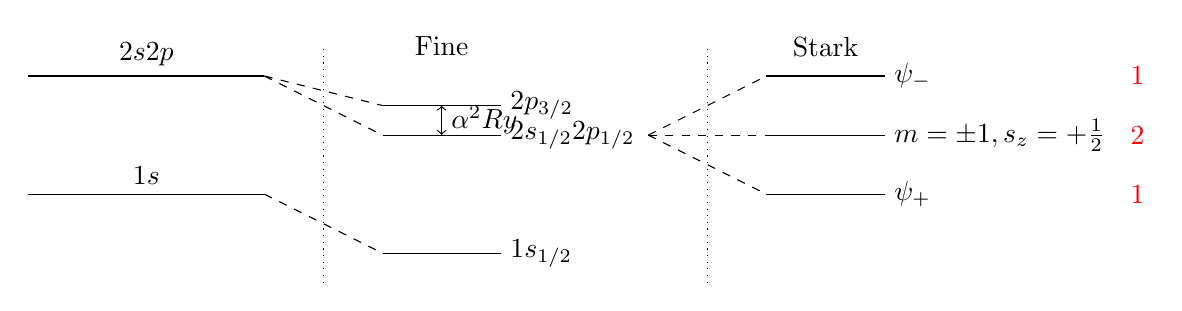
\begin{tikzpicture}[scale=1.5]
    \draw[] (0, 0) -- (2, 0);
    \draw[dashed] (2, 0) -- (3, -0.5);
    \draw[] (3, -0.5) -- (4, -0.5);
    \node[above] at (1, 0) {$1s$};
    \node[right] at (4, -0.5) {$1s_{1/2}$};
    
    \draw[] (0, 1) -- (2, 1);
    \draw[dashed] (2, 1) -- (3, 0.5);
    \draw[] (3, 0.5) -- (4, 0.5);
    \draw[dashed] (2, 1) -- (3, 0.75);
    \draw[] (3, 0.75) -- (4, 0.75);
    \node[above] at (1, 1) {$2s2p$};
    \node[right] at (4, 0.5) {$2s_{1/2}2p_{1/2}$};
    \node[right] at (4, 0.75) {$2p_{3/2}$};
    \draw[<->] (3.5, 0.5) -- (3.5, 0.75);
    \node[right] at (3.5, 0.625) {$\alpha^2\si{Ry}$};
    \draw[dotted] (2.5, -0.75) -- (2.5, 1.25);
    \node[] at (3.5, 1.25) {Fine};
    
    \draw[dashed] (5.25, 0.5) -- (6.25, 1);
    \draw[dashed] (5.25, 0.5) -- (6.25, 0);
    \draw[dashed] (5.25, 0.5) -- (6.25, 0.5);
    \draw[] (6.25, 1) -- (7.25, 1);
    \draw[] (6.25, 0) -- (7.25, 0);
    \draw[] (6.25, 0.5) -- (7.25, 0.5);
    \draw[dotted] (5.75, -0.75) -- (5.75, 1.25);
    \node[right] at (7.25, 1) {$\psi_-$};
    \node[right] at (7.25, 0.5) {$m = \pm 1, s_z = +\frac{1}{2}$};
    \node[right] at (7.25, 0) {$\psi_+$};
    \node[right, red] at (9.25, 1) {$1$};
    \node[right, red] at (9.25, 0.5) {$2$};
    \node[right, red] at (9.25, 0) {$1$};
    \node[] at (6.75, 1.25) {Stark};
\end{tikzpicture}
\end{document}